\newpage
\section{O Programa}

Para a implementação do algoritmo fora concebido um programa em C, ele inicializa os pesos e o bias com valores entre 0 e 1 para cada treinamento, que é feito utilizando os valores já predefinidos. A taxa de aprendizado escolhida foi de 0.0025 e a Precisão de $10^{-6}$. Após o treino podemos escolher fazer outro ou testar a rede (para valores já predefinidos também), e o programa fornece um gráfico do erro quadrático em função dos ciclos.


\begin{figure}[H]
	\centering
	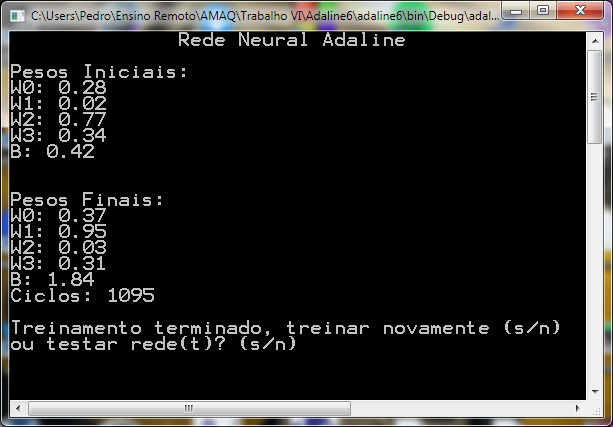
\includegraphics[scale = 0.9]{imagens/interface}
	\caption{Interface do programa.}
\end{figure}

\section{Resultados}

Realizamos cinco treinamentos em série, e estes foram os resultados obtidos para cada um deles:

\begin{figure}[H]
	\centering
	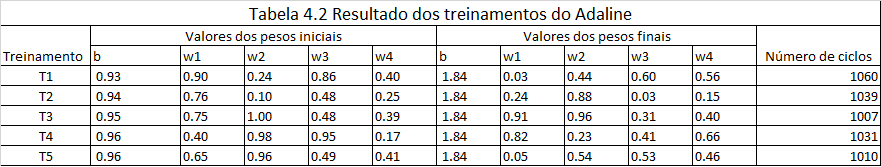
\includegraphics[scale = 0.7]{imagens/tabela4.2}
	\caption{Resultados para cinco treinamentos.}
\end{figure}

Os gráficos dos dois primeiros erros quadráticos foram plotados, observemos como são idênticos, isso significa que a rede tem um bom comportamento, em ambos o erro tende a 5.


\begin{figure}[!htb]
	\centering
	\begin{minipage}{0.5\textwidth}
		\centering
		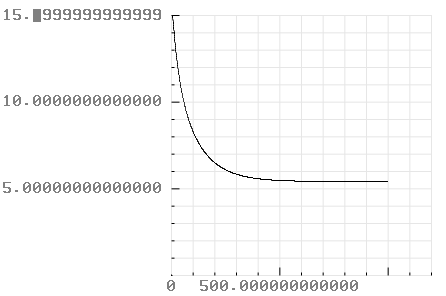
\includegraphics[scale = 0.5]{imagens/G1}
		\caption{Gráfico do Erro\\ Quadrático para o treinamento t1.}
		\label{fig:prob1_6_2}
	\end{minipage}%
	\begin{minipage}{0.5\textwidth}
		\centering
		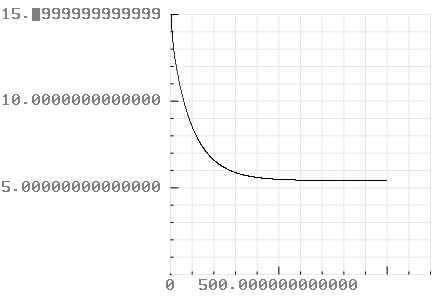
\includegraphics[scale = 0.5]{imagens/G2}
		\caption{Gráfico do Erro\\ Quadrático para o treinamento t2.}
		\label{fig:prob1_6_1}
	\end{minipage}
\end{figure}

Finalmente, a rede foi testada para os valores predefinidos como se vê na tabela abaixo, todos os resultados foram iguais, então temos uma rede bem treinada com resultados satisfatórios.

\begin{figure}[H]
	\centering
	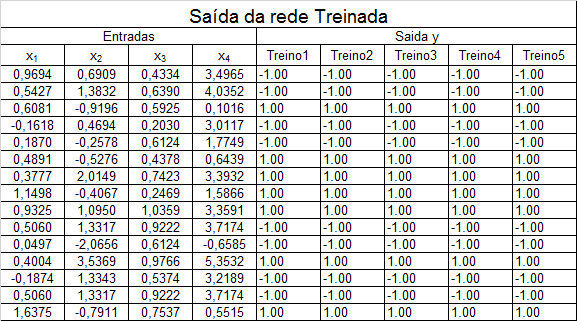
\includegraphics[scale = 1]{imagens/saida}
	\caption{Tabela com as entradas e saídas do teste para a rede já treinada.}
\end{figure}